\section{Methodology, ethics, and repeatability of case studies} \label{section-methodology-ethics-and-repeatability-of-case-studies}

\begin{figure}
    \centering
    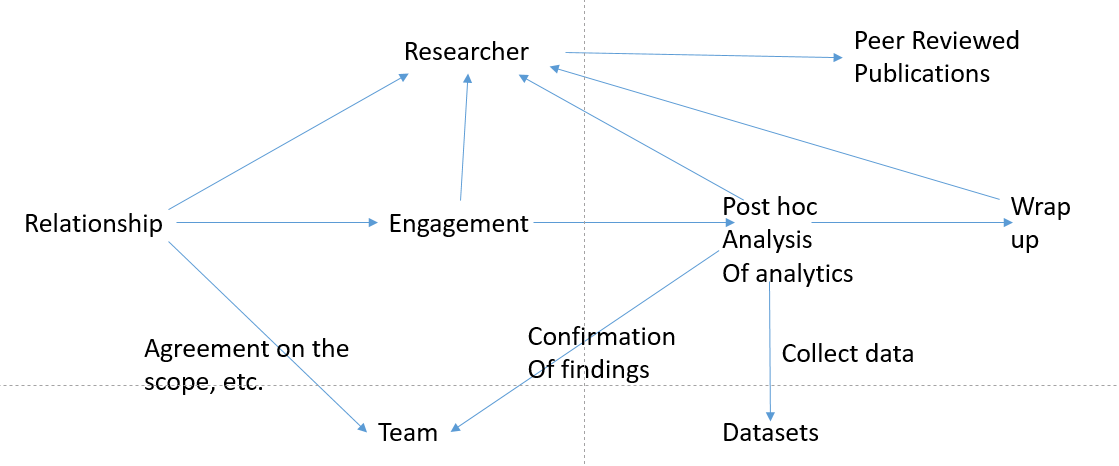
\includegraphics[width=14cm]{images/rough-sketches/Yijun-rough-sketch-of-relationships-in-case-study-methodology.png}
    \caption{Yijun's rough sketch of the methodology- a w-i-p}
    \label{fig:yijun-methodology-sketch}
\end{figure}




\subsection{Repeatability}
\textbf{Expand on:} What's hard to repeat (and why), aims to improve and demonstrate repeatability of the practices applied in this research.
\textbf{Absolutely key is what another researcher would do.}

One objective is to make the \emph{post-hoc} analysis repeatable, where others can perform the analysis and obtain similar results; therefore this section explains various patterns of analysis and there are various worked examples provided in the individual case studies.

\isabel{suggests repeatability is part of good research ethics.}
\isabel{Research as a political statement c.f. her transfer report.}

\begin{comment}
TODO papers to consider discussing here include: 
\begin{itemize}
    \item ``R3: repeatability, reproducibility and rigor"~\citep{vivek2012_r3_repeatability_reproducibility_and_rigor}

\end{itemize}
\end{comment}


\subsection{Research ethics for the case studies}
\label{section-research-ethics-for-the-case-studies}
The majority of the case studies presented in this research include other people. It is right and proper to ensure they and their respective organisations are willing to support the research directly - by participating - and/or indirectly - for instance by providing access to systems, tools, bug tracking systems, and so on. Some organisations require non disclosure agreements, and - in practice - they all choose what access to provide to what, to whom, and for how long. 

Engagement and trust need to be established with the people who manage the project and with the people who participate in the case study. Organisations often require approval from one or more senior representatives in the organisation, these may include head of development, and one or more of their legal, marketing, commercial, and risk departments.

For startups, one person may hold multiple roles, for instance in small startup teams they may be the CTO while also being an active developer of the software, \emph{and} the person responsible for operations, support and customer service. This was the case for two of the case studies presented in this research (LocalHalo and Iteratively), and in Moodspace the CTO was also the main developer of the app. In terms of obtaining permission, startups tend to be easy to work with if they agree to support the research as one or two people can quickly decide to support the research and provide access to whatever materials they are willing to share. They may not have time or patience to read or sign formal agreements, however an email summary of any verbal agreement helps to sum up that agreement and provide them the opportunity to confirm, clarify, or reject the contents of the agreement.

Mutualism, commensalism, parasitism, predation and competition are five types of symbiotic relationship. % ``There are five main symbiotic relationships: mutualism, commensalism, predation, parasitism, and competition."  Symbiosis: The Art of Living Together https://www.nationalgeographic.org/article/symbiosis-art-living-together/ 
Of these the last three may produce adverse outcomes for at least one participant.
In computer science research that involves organisations and live projects the type or types of symbiotic relationship(s) are another key consideration. The candidate projects and their organisations need to be confident that if they participate as case studies in research that they will not suffer in the relationship. If they see mutual benefits of the research they may be more willing to actively participate. 

As \citet[p.2]{robinson2019_applying_endosymbiosis_theory_tourism_and_its_young_workers} observe: \emph{``Business, or work, ecosystems are a community of interacting organisations and individuals (or groups) – or the organisms of the commercial world"}. Their research was into the relationships of Tourism and its young workers, and the possibility for exploitation in either or both directions. The challenges in their domain may apply to this type of case study based research and the researcher is wise to consider the potential adverse effects for any of the parties involved in the case study.

Another consideration is the concept of `agency' that the organisations and the relevant people are free to choose whether they wished to participate in the research. Some candidates declined to participate in the research on behalf of their project or organisation for various reasons. A common reason was lack of time on their part, another was that some candidates perceived the research would not be acceptable to their organisation, for instance owing to confidentiality or business risk.

The participants choose their model of engagement, this means the research needs to be adapted to their engagement model, availability, and ways of working. The researcher may need to bridge between and/or mediate between the academic research ways of working and those practiced in industry, and here in the domain of mobile app development. In particular the researcher needs to uphold the expectations of both academia and industry, this may be easier for someone who has sufficient experience and competence in both ecosysystems.

\newthought{How were these research concepts applied in this research?}
Every one of the actual case studies, and those that did not come to pass, started with a connection between two or more people. Sometimes the connection was indirect via someone who knew of the research. In several cases the relationship was established by someone at the candidate case study who was aware of the researcher and the research. There will be other ways to recruit potential case studies, however they were not used for this research.

However an initial contact/communication came about thumbnail of the research was presented to the candidate. This included an explanation that at least some of the work would need to be permitted to be published as part of the research and that permission would need to be freely given. With the exception of a particular commercial case study the engagement was voluntary and unpaid. The particular commercial case study ran alongside a paid consultancy where the researcher was engaged to help address challenges in one or more projects with similar aims to this research. Details of the organisation, the project(s), and the particular results are constrained by a commercial non-disclosure agreement.

For the two direct engagement case studies for opensource projects, they both asked for help to improve the reliability of at least one of their Android apps. Therefore the engagement had the potential to be mutually beneficial. Similarly, for the case studies with mobile analytics tool/service providers they saw value in being engaged with the research and the immediate results of those case studies. For the developer interviews the symbiotic relationship was closest to being commensal, while they may glean some benefits, it was not a primary factor in their willingness to participate. Instead they were keen and willing to help with the research for the good of the research. 



\begin{itemize}
    \item Ethics review for Workshop in Poland (and then for various reasons the contents of the workshop were not viable because of the effects of COVID-19.
    \item No other human subjects, the data related to apps and how the app is used and performs, humans are not the subject of the research.
    \item Opensource, freely available apps without any restrictions on sharing the findings of the performance of the apps. No PII information collected by the analytics tools used.
    \item Semi-structured interviews with various individuals in their professional and/or project capacities.
\end{itemize}

Participants were briefed and gave their permission either individually or on behalf of their organisations to use the material they freely provided. Several have reviewed my research and provided constructive feedback which has been applied. 
It has not always been practical to reach them, for instance some are no longer reachable. None of the analytics information provided contains PII.

Some of the opensource projects that form part of this research received and accepted pull requests from the researcher, these were freely given and freely received and have no known monetary value.

\begin{comment}
TODO papers to consider discussing in the ethics section include: 
\begin{itemize}
    \item ``The human is the loop: new directions for visual analytics"~\citep{endert2014_the_human_in_the_loop_new_directions_for_visual_analytics}
    \item ``Not All Trust Is Created Equal: Dispositional and History-Based Trust in Human-Automation Interactions"~\citep{merritt2008_not_all_trust_is_created_equal_etc}.
    \item \emph{``Symbiosis
Symbiosis refers to the partnership (usually long-term) that is established between two or more organisms. In microbiology, symbiotic relationships are often established between a microorganism and its host, and the partnership can be mutualistic or parasitic."} \url{https://www.nature.com/subjects/symbiosis}
\end{itemize}
\end{comment}

\clearpage